
\documentclass[12pt,a4paper,oneside]{article}
\usepackage[margin=1.2in]{geometry}
\usepackage{appendix}
\usepackage[dvips]{graphicx}
\usepackage{epsfig}
\usepackage{amsmath}
\usepackage{amssymb}
\usepackage{psfrag}
\usepackage[square, comma,sort,numbers]{natbib}
\usepackage{fancyhdr}
\usepackage[nottoc]{tocbibind}
\usepackage{color}
\usepackage{fixltx2e}
\usepackage{pdfpages}
\usepackage{pdflscape}
\usepackage{booktabs}
\usepackage{graphicx}
\usepackage{float}
\usepackage{afterpage}
\usepackage{subcaption}
\usepackage{lscape}
\usepackage{rotating}
\usepackage{enumitem}
\usepackage{array,tabularx}
\usepackage{fancyref}
\usepackage[dvipsnames]{xcolor}
\usepackage[colorlinks=true,allcolors=blue]{hyperref}%



\newcommand{\quotes}[1]{``#1''}

\newenvironment{conditions*}
  {\par\vspace{\abovedisplayskip}\noindent
   \tabularx{\columnwidth}{>{$}l<{$} @{\ : } >{\raggedright\arraybackslash}X}}
  {\endtabularx\par\vspace{\belowdisplayskip}}



\pagestyle{fancy}
\title{\Huge The Hat Creek Radio Observatory\\
\vspace{0.5cm}
The IF Splitter\\
\vspace{0.5cm}
\normalsize \emph{}
\vspace{3.5cm}
\begin{center}

\includegraphics[height=4cm]{titlepage/SETI_institute_logo.jpg}
\end{center}
}
\author{ 
\vspace{1cm}
\Large
\textbf{ Alexander Pollak \& Marc Jacquart} \\
SETI Institute \\ 
189 Bernardo Ave, Suite 200 \\
Mountain View, CA 94043 \\ 
Alexander.Pollak.87@gmail.com\\
}
\date{\today}



\begin{document}
\clearpage\maketitle
\thispagestyle{empty}

%\newpage
%\thispagestyle{empty}
%\section*{Abstract}
%\noindent 
%



%
%\vspace{3cm}
%\begin{flushright}
%Alexander Pollak \\ \emph{September, 2015}
%\end{flushright}

%\newpage
%\thispagestyle{empty}
%\tableofcontents
\newpage

%----------------------------------------------------------------------------------------
%	General
%----------------------------------------------------------------------------------------
%\pagestyle{plain}
\section{General}
\label{sec:General}
% ----------------------------------------------------------------

This document outlines general information regarding the IF Splitter such as the design, parts, wiring, cabling, and testing. This information is aimed at detailing the entire process of creating an IF Splitter from design to manufacturing to testing. 


%----------------------------------------------------------------------------------------
%	CAD Design and Drawings
%--------------------------------------------------------------------------------------

\section{CAD Design and Drawings}
\label{sec:CAD}
% ----------------------------------------------------------------
This section includes a description of the CAD design.

\hfill \break

%
%\begin{figure}[H]
%\centering
%\includegraphics[width=1\linewidth]{<path>/picture.png}
%\caption{Caption}
%\label{fig:LABEL}
%\end{figure}
%


\subsection{Design}
\label{sec:Design}
% ----------------------------------------------------------------
Different parts

%--
\subsection{Wiring}
\label{sec:Wiring}
% ----------------------------------------------------------------


\subsection{Testing}
\label{sec:Testing}
% ----------------------------------------------------------------

%----------------------------------------------------------------------------------------
%	Power Supplies & Adapter
%----------------------------------------------------------------------------------------
\section{Power Supplies \& Adapter}
\label{sec:Power}
% ----------------------------------------------------------------

%----------------------------------------------------------------------------------------
%	Module Wiring
%--------------------------------------------------------------------------------------


\subsection{Front Panel}      
\label{sec:FrontPannel}
% ----------------------------------------------------------------

%----------------------------------------------------------------------------------------
%	Module Testing
%----------------------------------------------------------------------------------------
\section{Testing}
\label{sec:Testing}
% ----------------------------------------------------------------


\subsection{Setup}
\label{sec:Testing_Setup}
% ----------------------------------------------------------------


\subsection{Method \& Desired Results}
\label{sec:Testing_Method}
% ----------------------------------------------------------------

\subsection{Troubleshooting}
\label{sec:Testing_Troubleshooting}
% ----------------------------------------------------------------

 \newpage
 
%----------------------------------------------------------------------------------------
%	Appendix A: Attemplifier Module Enclosure Drawings
%----------------------------------------------------------------------------------------

\appendix
% ----------------------------------------------------------------

% To include pages from other PDFs
% 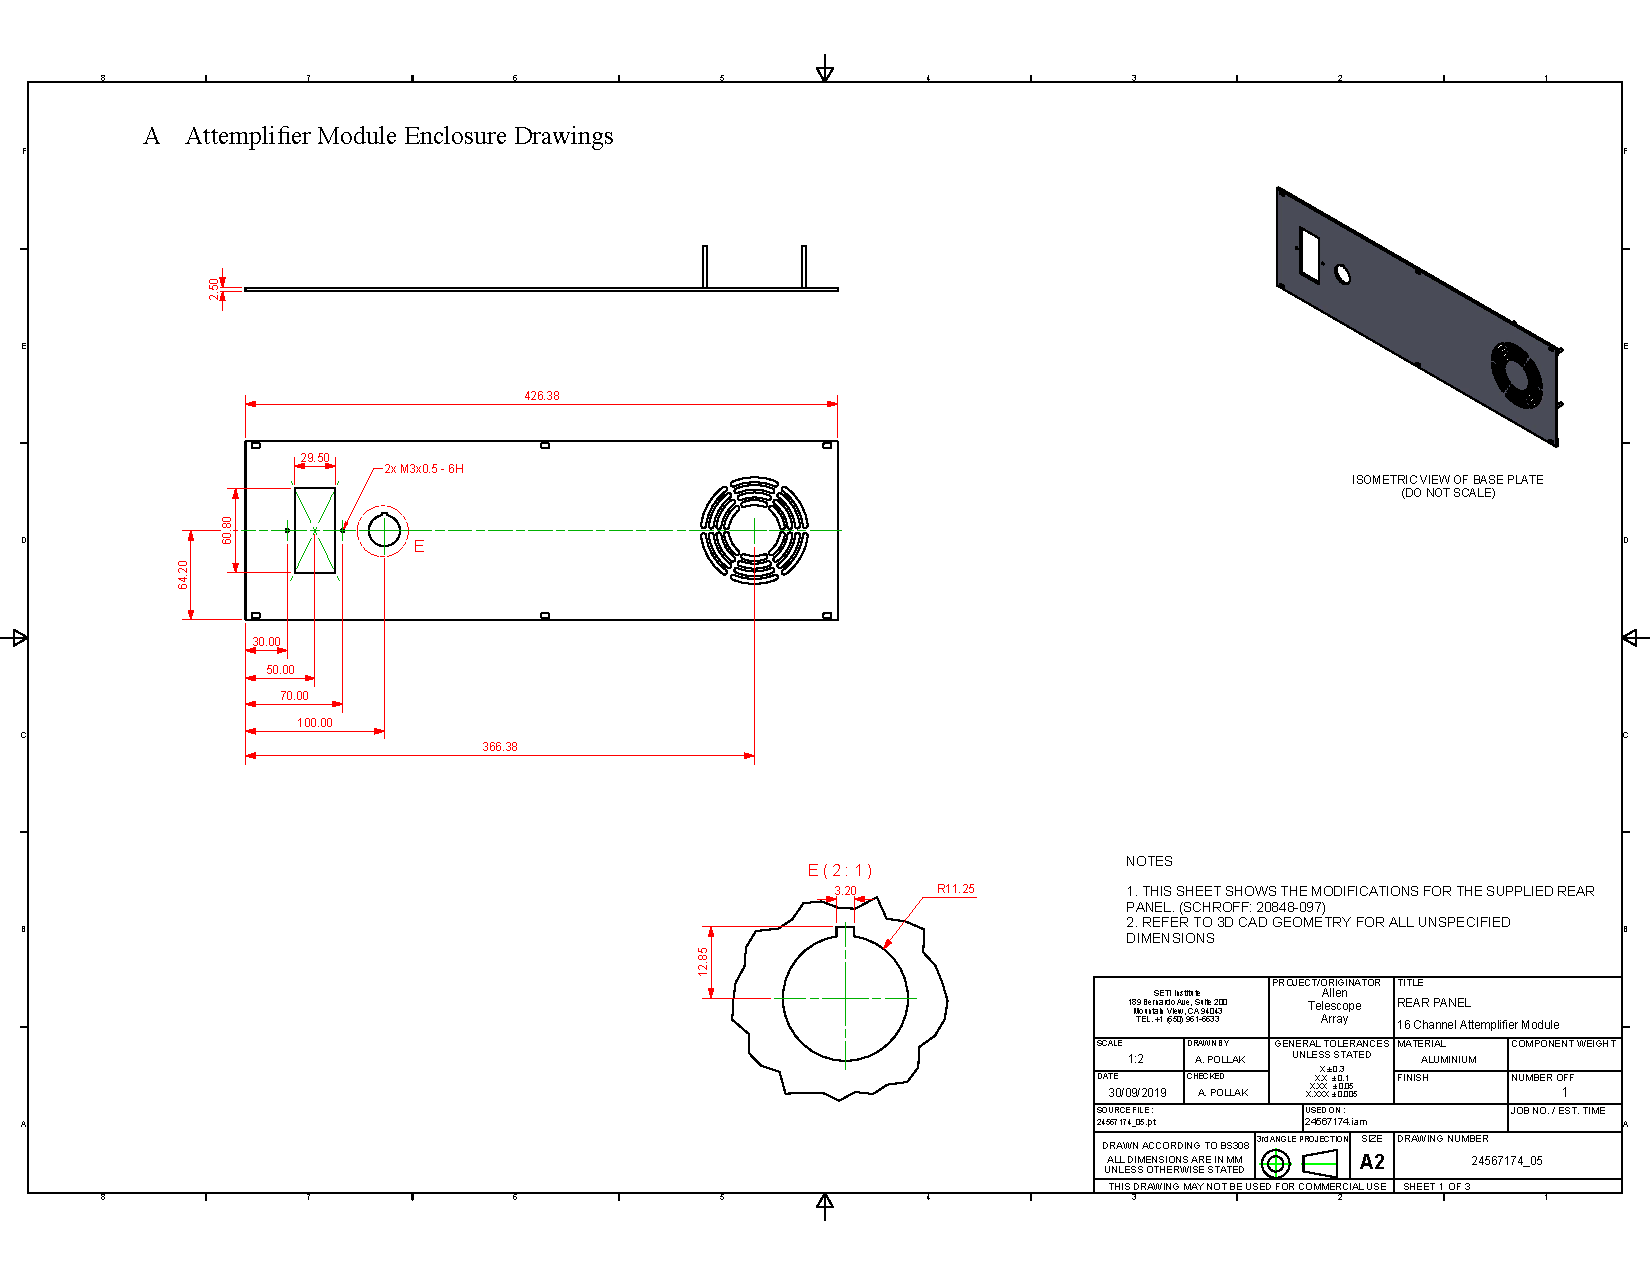
\includepdf[pages=-, landscape=true]{Documentation/PDFs/24567174_05(copy).pdf}


%----------------------------------------------------------------------------------------
%	Appendix B: Attemplifier Module Component List
%----------------------------------------------------------------------------------------
\begin{landscape}
\section*{B \hspace{.5cm} Component List of Attemplifier Module}

% ----------------------------------------------------------------

\begin{table}[H]
\centering
\resizebox{1.5\textwidth}{!}{%
\begin{tabular}{@{}lllllll@{}}
\toprule
Qty & Unit & Description & Manufacturer & PN Manufacturer & Distributor & PN Distributor\\
\midrule
1 & Each/Pack & & & &\\


\bottomrule            
\end{tabular}}
\label{tab:Attemp_components}
\end{table}

%----------------------------------------------------------------------------------------
%	Appendix D: Control Board Schematics
%----------------------------------------------------------------------------------------

\section*{D \hspace{.5cm} Control Board Schematics}

% ----------------------------------------------------------------

%
%\begin{figure}[H]
%\centering
%\includegraphics[width=1\linewidth]{<path>/picture.png}
%\caption{Caption}
%\label{fig:LABEL}
%\end{figure}
%

\end{landscape}

%----------------------------------------------------------------------------------------
%	Appendix E: Attemplifier Enclosure Drawings
%----------------------------------------------------------------------------------------
\begin{landscape}
\section*{E \hspace{.5cm} Attemplifier Enclosure Drawings}

% ----------------------------------------------------------------

%
%\begin{figure}[H]
%\centering
%\includegraphics[width=1\linewidth]{<path>/picture.png}
%\caption{Caption}
%\label{fig:LABEL}
%\end{figure}
%
\end{landscape}
\end{document}
